% !TEX encoding = UTF-8 Unicode
% !TEX program = pdflatex
% !TEX spellcheck = en_US


% In order to correctly compile this document,
% execute the following commands:
% 1. pdflatex
% 2. pdflatex
% 3. pdflatex



\documentclass[amsthm,ebook]{saparticle}

% IF YOU USE PDFLATEX
\usepackage[utf8x]{inputenc}

\usepackage[normalem]{ulem}
% if you write in english and in greek
\usepackage{ucs}
\usepackage[greek,english]{babel}
\usepackage{teubner}
\languageattribute{greek}{polutoniko}



% IF YOU USE XELATEX
%\usepackage{polyglossia}
% if you write in italian
%\setmainlanguage{italian}
% If you want put some ancient greek:
%\setotherlanguage[variant=polytonic]{greek}
%\newfontfamily{\greekfont}[Ligatures=TeX]{Palatino Linotype}

% dummy text (remove in a normal thesis)
% remove if not necessary
%\usepackage{siunitx}
%Natbib for bibliography management
\usepackage[authoryear]{natbib}
% custom commands
\newcommand{\bs}{\textbackslash}

%%%%%%%%
%TITLE:%
%%%%%%%%
\title{Teaching (Digital) Epigraphy}
\author[ilc]{Marion Lamé}
\author[zag]{Ivan Radman-Livaja}
\author[mau]{Bruce Robertson}
\author[isti]{Federico Ponchio\corref{first}}
\address[ilc]{Istituto di Linguistica Computazionale}
\address[isti]{Visual Computing Laboratory, ISTI-CNR}
\address[zag]{Archaeological Museum in Zagreb}
\address[mau]{Mount Allison University}
\cortext[first]{Corresponding author. Email: federico.ponchio@isti.cnr.it}

\date{2015-12-02}
\begin{document}

\maketitle
\begin{abstract}
Although having the experience of directly manipulating an ancient text-bearing artifact is important for developing the
skills of an epigrapher – an experience that books and photo cannot replace – such access to primary sources is often
problematic. In this article we present our experience with teaching students to transcribe and interpret Roman
inscribed lead tags, using a Digital Autoptic Process (DAP) in a web environment, so to develop basic competences in
epigraphy and digital epigraphy.
\end{abstract}
\keywords{Educational project, digital epigraphy, epigraphy, open access, primary sources}

\section{Introduction}

\noindent Although undergraduate students are naturally attracted to inscriptions and epigraphy affords them an important window
on the past, they are seldom given the opportunity to study inscriptions directly. This is because epigraphical work is
seen as the specialist’s domain: the analysis of such material generally requires a rather high level of expertise,
normally acquired during graduate studies and beyond. Lacking sufficient skills and knowledge to comprehensively
understand often complex epigraphic data, undergraduate students are simply unable to offer the expert opinions
sometimes sought by a project manager. Thus, offering undergraduate students the opportunity to tackle tasks usually
reserved to their senior colleagues is certainly not a common occurrence. In our small project ``Pedagogical,
Scientific \& Technical Experiment in Digital Epigraphy: the Study Case of the \emph{Tesserarum Sisciae Sylloge} (TSS) through
a Digital Autoptic Process (DAP)'' we aimed to challenge this state of affairs. Using digital methods and a
custom-designed course of rapid study, we offered undergraduates the opportunity to tackle epigraphic tasks usually
reserved to their senior colleagues. We made use of newly-digitized epigraphic material: Roman commercial lead tags
from the ancient city of Siscia.

\section{Epigraphic Primary Sources of Information}


\noindent The Roman Department of the Archaeological Museum in Zagreb (AMZ) contains close to 1200 of these inscribed lead tags
found in Sisak (Siscia), one of the largest urban centers in south-western Pannonia. Most of them were found during the
dredging of the Kupa river before WWI. Since the dredging was localized in the very centre of the town, i.e. in front
of the old Roman port quarter, it would seem that all the tags come from a limited area. All of those tags are small
lead tablets, of a more or less rectangular shape, pierced with a hole so that the tag could be attached to the bags
containing the merchandise or to the merchandise itself with a small rope or a metal wire. They all carry an
inscription, most of the time on both sides. Those inscriptions are always, up to now, written in capital letters or
the older Roman cursive, sometimes even in a mixture of both. Most of the tags were reused several times and thus they
carry traces of older inscriptions (palimpsests). Those inscriptions usually follow the same model: one side of the tag
carries personal names, the other side carries an inscription mentioning the merchandise, most of the time in an
abbreviated form, as well as a price - normally expressed in \emph{denarii} or fractions of the \emph{denarius} - and quite often an
indication of quantity or weight.

\begin{figure}[!h]
\centering
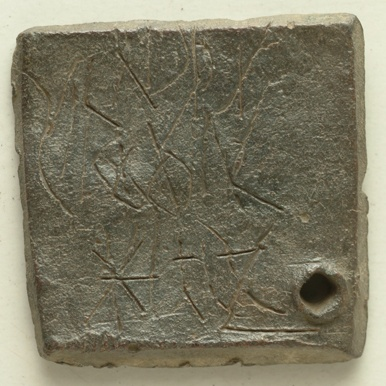
\includegraphics[scale=0.25]{EAGLE16lameetalteaching-img001.jpg}
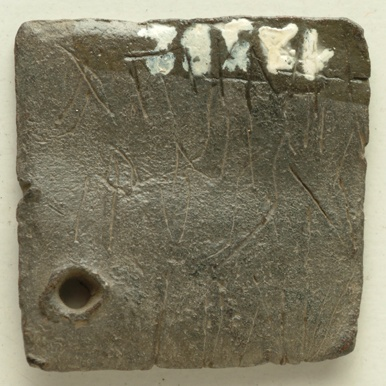
\includegraphics[scale=0.25]{EAGLE16lameetalteaching-img002.jpg}
\caption{No. 12582.}
\label{fig:12582}
\end{figure}

A traditional print photograph, such as this one (No. 12582, Fig.~\ref{fig:12582}) drawn from the archives of the AMZ, limits the student’s
opportunity to learn to decipher these tags. Even if a professional photographer took this picture with a good quality
camera in a fully equipped photographic studio, the reading of the inscription stays riddled with uncertainties and a
researcher would have to check the tag \emph{de visu} in order to offer a plausible transcription.

\begin{figure}
\centering

\end{figure}
Most of the tags, if not all, are linked to the wool trade and the textile industry. Words like \emph{LANA, PAN(N)UM, TVNICA, SAGVM, P(A)ENVLA, PAL(L)A, PALLIOLUM, LODIX, BANATA}, and \emph{ABOLLA}, appear regularly enough without being abbreviated and
thus the interpretation of common abbreviations like \emph{l, la, lan, pan, t, sag, paenv, pal, lo, lod, lodi, bana, ab} is
not in doubt. The other abbreviations are mostly related to terms of colour. The prices on those tags are an important
information: they indicated the value of the goods or the cost of a given service (e.g. cleaning, fulling, dyeing). It
would also appear that they were used by fullers and dyers as ownership tags. By noting the name of the client as well
as the type of cloth or service and the price on the tag which was subsequently attached to the item to be processed
(i.e. cleaned or dyed), shop owners could easily return their property to the clients as well as charge them the
correct fee\footnote{\citet{radman_livaja_segestica_2008}, \citet{radman-livaja_roetiquettes_2010}, \citet{radman-livaja_5_2013}, \citet[165-172]{radman-livaja_two_2013}, \citet{radman-livaja_plombs_2014},  for analogous tags with \citet[97-104]{mocsy_olom_1956}; \citet[195-210]{egger_funf_1968}; \citet[127-138]{frei-stolba_les_2011}; \citet[121-137/93, 215-222]{schwinden_romerzeitliche_1985}; \citet{romer-martijnse_romerzeitliche_1990}; \citet[5-48]{romer-martijnse_fruhkaiserzeitliche_1997}; \citet[301-305]{feugere_etiquette_1993}; \citet[211-220]{weiss_bleietiketten_1991}; \citet[29-40]{paci_etichette_1995}; \citet[207-216]{bassi_tre_1996}; \citet[121-135]{bizzarini_quattro_2005}; \citet[43-51]{buchi_etichette_2005}; \citet[42-110]{cresci_supellex_2010}; \citet[295-317]{jacques_artisanat_2010}; \citet[237-246]{wedenig_bleietikett_2013}.}. 

Some of the genuine difficulties of the autoptic process are already solved by a static picture in a print publication.
The tag has a given position, it is illuminated from one direction only and therefore it already suggests a reading
direction. A DAP should be able to confront the students to some of those difficulties and to overcome them alone.

In order to consider the value and usefulness of the DAP in this particular case study, the fact that some of the
students had not yet a real background in Latin paleography was actually more of an asset. Indeed, if untrained
students with few basic skills can use the digital edition as a specific medium without too much difficulty, albeit
under supervision of specialists (Digital Epigraphy, Ancient History, Archaeology, Epigraphy, \ Computer Graphics and
Digital Humanities) then the whole concept would appear as convenient and appropriate for similar case studies and
research. 

\section{Digital Epigraphy}


\noindent In fact, the transcription and interpretation of Roman inscribed lead tags are often challenging, and so we ignored how
far we could go with these students if useable results would ensue. First we made a selection of fourty tags to be
subjected to the adequate digitization process we chose to work with: Reflectance Transforming Imaging (RTI). It is a
small but nevertheless representative sample of the whole corpus. The students had at their disposal different kinds of
inscriptions, including both easily readable specimens and more challenging graffiti (e.g., No. 12582). One may also
profit from the assistance of undergraduate and graduate students, which could not often be the case
before\footnote{\ The Laboratorio di Cultura Digitale, lead by Prof. Salvatori, at the University of Pisa applies the
didactic model DIGICRAFT. This means that undergraduate students might share their skills, especially the digital one,
in order to allow an entire team to reach its goal. For more information see: \url{http://www.labcd.unipi.it/laboratorio}.}.
This experiment showed that their contribution can be useful, because technology may compensate for their lack of
knowledge although the final conclusions have to remain in the domain of scholars familiar with the subject. In any
case, this experiment shows how the digital edition may allow both scholars and students to have an open access to what
is basically a primary source of information for humanities (presented as a digital facsimile)\footnote{\citet{gorman_opening_2015}
writes about some of the OA issues: ``While digitisation is not a pre-requisite to gaining access to material (...), and
while digital surrogates of cultural heritage objects do not have to be openly shared once created, just as the
sciences are calling for publication of source data as part of the Open Access movement, opening up access to primary
sources in the cultural heritage sector and encouraging them to be published in a way which is as accessible as
possible has the potential to change the nature of research outputs in the Humanities and Social Sciences, as well as
the nature of research itself in these areas.''}. Of course, learners could train themselves on the drawing of the tag,
but they would not confront the difficulty of interpreting the numerous ambiguities and the responsibility of deciding
what is on the tag. 

From a digital epigraphy standpoint, this consists of an online DAP \ modeled, in \citet{Lame2015}, on a dispositive analysis
and the three fundamental systems of an inscription: writing system (wSystem), textual system (tSystem) and contextual
system (cSystem). Three tools compose the DAP: RTI web viewer, TSS viewer and MarkOut tool. The last two were
specifically designed for the digital edition of the corpus TSS. The following paragraphs present those three DAP
tools. Due to the material properties of the lead tags, it is impossible to capture the appearance of the letters with
a single image. When holding a tag it is necessary to change the light angle to enhance the different marks on the
surface. RTI is a computational photography technique that enables the interactive re-lighting of the observed object
from any light direction. This is accomplished combining into a single compact data structure a set of fixed camera
photographs taken under many different illumination conditions. The acquisition process is inexpensive and does not
require labor intensive steps, unlike 3d model acquisition. RTI visualization allows the user to virtually ‘tilt’ the
object and recreate different lighting conditions, mimicking part of the autoptic process. Another advantage is the
magnification provided by the high resolution camera employed. The widespread adoption in browsers of WebGL (Khronos
group 2009) recently enable RTI visualization on the web. We used the RTI web viewer developed by Visual Computing Lab,
ISTI-CNR. High resolution re-illuminable images allow the selection of the best view for each mark, thus allowing the
user to obtain an adequate readability of the lead tags through an intuitive interface. Another important advantage of
having the tags available online is that the students can easily compare a tag with any other tag already in the
database and compare occurrences of a letter in other already transcribed tags. Finally, the Web access facilitates the
discussion amongst students and experts worldwide.

The TSS viewer is used to give access to the raw and genuine data (115 photograms with different lighting angles) and
also to pick the best photo to be used in the linking tool MarkOut, while the RTI viewer can be consulted in parallel
to interactively relight the tag and examine problematic spots.

The drawing process consists in associating some heterogeneous elements of the wSystem and the tSystem. MarkOut is the
linking tool that allows to represent the graphico-textual (g/t) relationship between those two systems. MarkOut allows
the students to work on the wSystem of the inscriptions by drawing the signs over an image of the tag using the mouse.
The line is converted in a curve that can be later fixed using handles. Each mark, that represents a phenomenon of the
wSystem of the inscription, is assigned to some textual information such as a letter or a symbol (Unicode and/or XML
encoding), that represents a textual phenomenon of the tSystem of the inscription. This assignation creates inside the
MarkOut the g/t relationship used for query processing. The final result is an SVG file that can be easily parsed to
recover the linking information between wSystem and tSystem (e.g. browsing by glyph's shape and interpretation,
identifying glyph's position), and easily shared with anyone with a browser (e.g.: fig. \ref{fig:markout}). The linking tool MarkOut
is one of the editing components of the modular DAP. They fit into communication workflows\footnote{This raises, of
course, questions, most of them outside the purview of this article, about the relationship that evolves between
research and our modern societies. We invite the reader to peruse various initiatives such as \citet{bertocci_documenter_2006} on the «
valeur d'ancienneté » of cultural heritage, that participates to social well-being, the Civic Epistemologies
\url{http://www.civic-epistemologies.eu} and its Berlin charter, as well as Public History approaches
\url{http://public-history-weekly.oldenbourg-verlag.de}.} such as crowdsourcing, editing inscriptions, dialoguing with
experts, preserving and promoting cultural heritage and, as here, teaching some skills in epigraphy.


\begin{figure}[!bp]
\centering
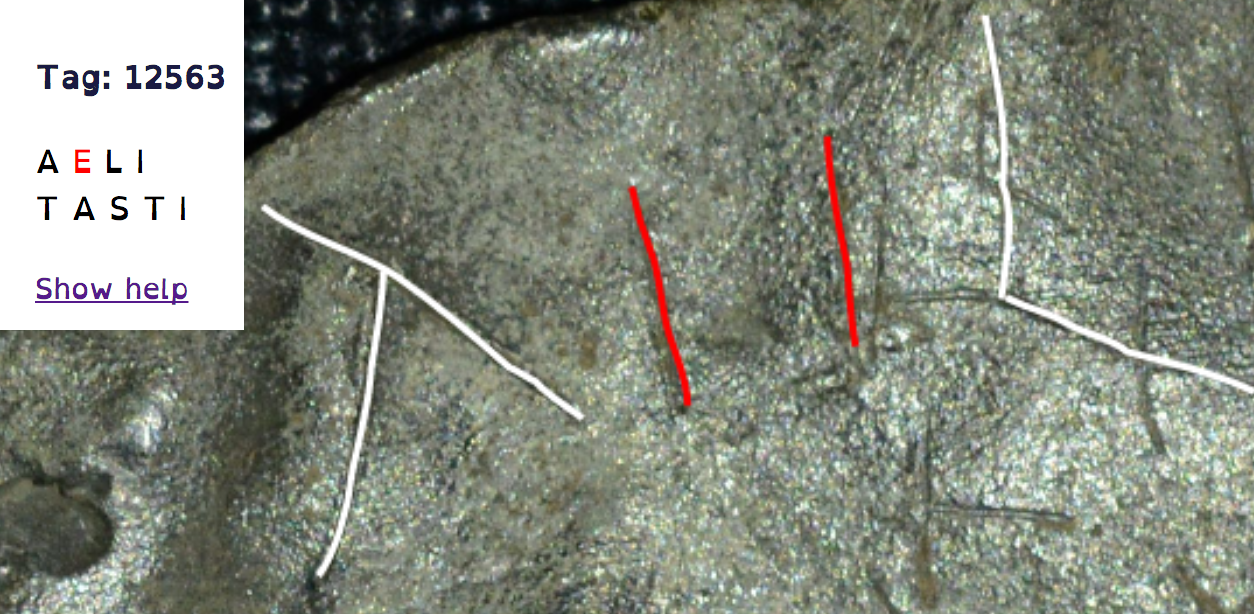
\includegraphics[scale=0.10]{EAGLE16lameetalteaching-img003.png}
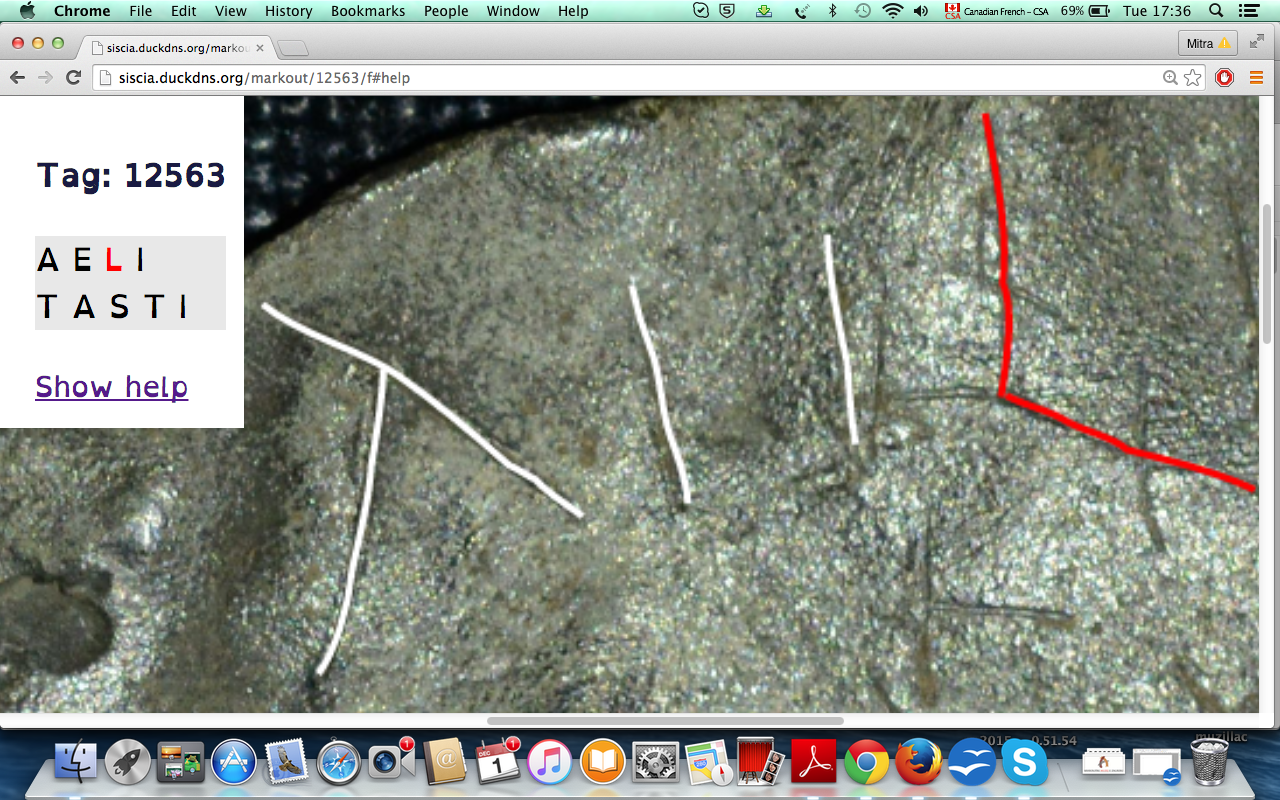
\includegraphics[scale=0.10]{EAGLE16lameetalteaching-img004.png}
\caption{MarkOut screenshots (detailed part of tag no. 12563) showing the association, expressed in red, of the Unicode
Latin characters with the position and the shape of the writing: U+0045 with II (identified as E2 by students) and
U+004C with L (L1 or L5).}
\label{fig:markout}
\end{figure}

Students were involved for a very short period of time: on average two hours per day over a couple of days only (in
Spring 2014 and in Fall 2015). This training was delivered in three steps (``Readings'', ``Writings'', ``Test \& Taste a
DAP'') during which there were given some academic documentation about the lead tags, and basic knowledge about digital
epigraphy (epigraphic message in a computer, dispositive analysis, existing projects, digital tools, XML and Unicode
encoding, DAP, and issues regarding digital representation of artifacts).

Students encountered their first epigraphic challenges with tag no. 12582 \citep[cat 03.13, 347]{radman-livaja_plombs_2014}, found in
the Kupa river in Sisak and offered by Andrija Colussi to the Archaeological Museum in 1898. It is a rather typical
lead tag of an irregular rectangular form, pierced with a hole. Its size (22.7x22.8x2.4 mm) corresponds fairly well to
the average size of other specimens found in Siscia. Although its surface is rather damaged and shows clear traces of
erasure, the most recent inscription remains quite readable. However, many traces of an older record (or several older
records?), complicate significantly the transcription and the interpretation. The last inscription can be read,
nevertheless, but it demands a certain effort and quite a lot of experience in Latin palaeography:

\begin{minipage}[t]{0.25\textwidth}
\textbf{Obverse}\\
At\d{e}\d{r}\\
ivs
\end{minipage}
\begin{minipage}[t]{0.25\textwidth}
(palimpsest)\\
\d{S}\d{i}\d{i}\d{x}\d{t}\d{i}\\
i onis n\\
i . n i 
\end{minipage}
\begin{minipage}[c]{0.30\textwidth}
%\begin{figure}
%\centering
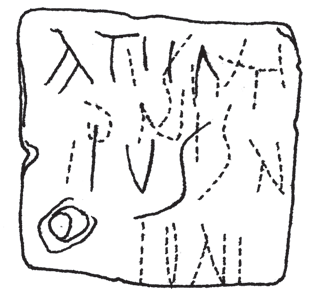
\includegraphics[width=2.965cm,height=1.79cm]{EAGLE16lameetalteaching-img005a.png}
%\end{figure}
\end{minipage}

\begin{minipage}[t]{0.25\textwidth}
\textbf{Reverse}\\
la(na) p(ondo) i\\
cor(ticea)\\
\sout{X} =-\pounds\\
\end{minipage}
\begin{minipage}[t]{0.25\textwidth}
(palimpsest)\\
. . . s\\
. . v\\
  iir 
\end{minipage}
\begin{minipage}[c]{0.30\textwidth}
%\begin{figure}
%\centering
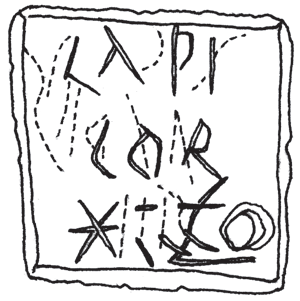
\includegraphics[width=2.845cm,height=1.896cm]{EAGLE16lameetalteaching-img005b.png}
%\end{figure}
\end{minipage}


The inscriptions on the obverse and reverse may not be contemporaneous and we may not affirm with confidence that the
individual named Aterius has something to do with the small quantity of wool mentioned on the obverse. The price is
rather low, since the value of the transaction appears to be only 1 sestertius and 1 dupondius, i.e. 6/16 of a
denarius. 

Traces of older inscriptions are hard to read and interpret but several personal names may be surmised. Such a tag was
particularly interesting for our experiment. It is quite a challenging inscription, even for a skilled epigraphist and
paleographer; we therefore were anxious to find out how efficiently the students would tackle it. Thanks to the DAP,
the transcription was not utterly difficult for most students. Obviously, in the first instance, the interpretation was
beyond their means, but we were nevertheless impressed by their abilities to read it far more easily than expected. The
DAP definitely offers the possibility to work on such material online, without the obligation to inspect it personally,
at least in the first stage.

Thus, students had to face similar issues as scholars who first tackled those epigraphic finds. However, the students
had one significant advantage, despite their lack of experience and skill. This major advantage was allowed by DAP
technologies, which considerably improved their odds. Despite their lack of elaborate knowledge on the subject, we
managed to train them to develop some necessary skills in order to be able to read the inscriptions as well as offer
meaningful transcriptions, thanks to the help of digital facsimiles. It was indeed really gratifying to observe their
enthusiasm during the experiment as well as their delight when they realized they could do it. Naturally, despite the
DAP, whatever the information technology may be, such scientific analysis still requires skilled scholars, but with the
help of technology, digital editions may be thoroughly checked and amended far more easily. Besides giving an
opportunity to further study the primary source of information and amend the paper editions and publications, it also
allows university teachers to train future scholars and specialists, wherever their geographic location may be. In this
particular case, the epigraphic material is in Croatia but the analysis was done online by scholars and students from
Canada, France, and Italy. We therefore believe that digital epigraphy has a role to fulfill in university teaching but
that one needs to establish right protocols and rigorous methods in order to warrant access to documents and ensure
further development of such teaching methods aiming to improve the formation of future specialists.



\section{Practicing Epigraphy}


\noindent Once alone, students were asked to ignore the monetary symbols then to decipher (with or without the help of
transcription and drawings) and to classify the written signs according to the following chart. Such preliminary
classification gives a first idea of the main general shapes one can find on a lead tag. It is not a paleographical
study, which has yet to be done, but it is efficient enough to train students at a first level of deciphering.

\subsection{Drawing With Help (No. 12563)}

\begin{minipage}[t]{0.18\textwidth}
\textbf{Obverse}\\
Aeli(i)\\
Tasti
\end{minipage}
\begin{minipage}[c]{0.27\textwidth}
%\begin{figure}
%\centering
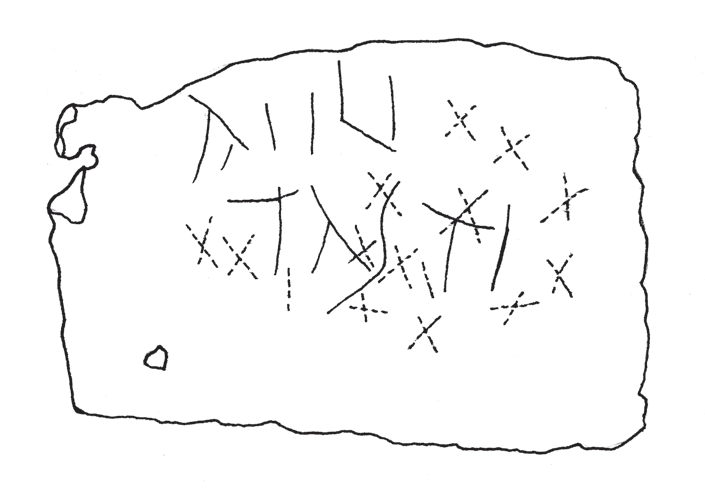
\includegraphics[width=2.965cm,height=1.79cm]{EAGLE16lameetalteaching-img006.png}
%\end{figure}
\end{minipage}
\begin{minipage}[t]{0.18\textwidth}
\textbf{Reverse}\\
\d{l}odicem\\
murtiola\d{m}\\
pondo vi s\\
\sout{X} vi s\\
\end{minipage}
\begin{minipage}[c]{0.25\textwidth}
%\begin{figure}
%\centering
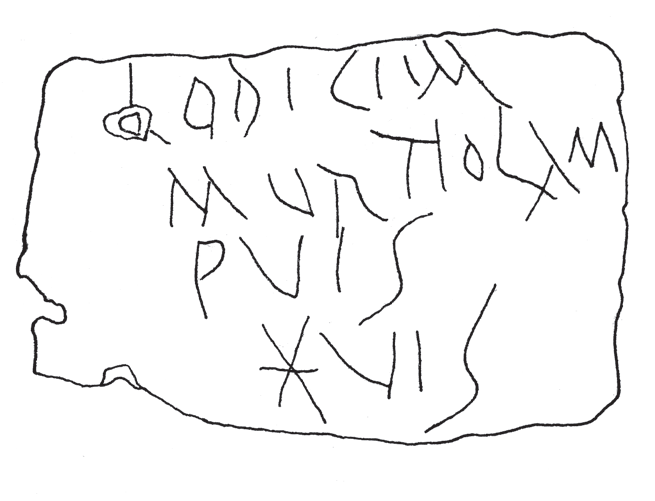
\includegraphics[width=2.845cm,height=1.896cm]{EAGLE16lameetalteaching-img007.png}
%\end{figure}
\end{minipage}



No. 12563 is a rectangular lead tag of irregular form with a badly damaged and scratched surface. Nevertheless, the most
recent inscription is clearly readable while one may still discern traces of older inscriptions. An older inscription
might be visible on the obverse, perhaps series of numbers but its meaning remains unclear. Students have
transcriptions and drawings.


\begin{table}
{\small
\addtolength{\tabcolsep}{-0.7mm}
\begin{tabular*}{\textwidth}{llllllllll}
\toprule
\textbf{12563 (obv)} & \textbf{A} & \textbf{E} & \textbf{L} & \textbf{I} & \textbf{T} & \textbf{A} & \textbf{S} & \textbf{T} & \textbf{I}\\
\midrule
\textbf{Stud. 1} & \textit{A10} & \textit{E2} & \textit{L11} & \textit{I1} & \textit{T1} & \textit{A10} & \textit{S3} & \textit{T2} & \textit{I1} \\
\textbf{Stud. 2} & \textit{A10} & \textit{E2} & \textit{L5} & \textit{I1} & \textit{T2} & \textit{A10} & \textit{S4?} & \textit{T2} & \textit{I1}  \\
\bottomrule
\end{tabular*}

\begin{tabular*}{\textwidth}{llllllllllllll}
 & & & & & & & & & & & & & \\
\toprule
\textbf{12563 (rev)} & \textbf{L} & \textbf{O} & \textbf{D} & \textbf{I} & \textbf{C} & \textbf{E} & \textbf{M} & & & & & &\\
\midrule
\textbf{Stud. 1} & \textit{L2} & \textit{O3} & \textit{D3} & \textit{I1} & \textit{C2} & \textit{E2} & \textit{M5} &  &  & & & & \\
\textbf{Stud. 2} & \textit{?} & \textit{O3} & \textit{D5} & \textit{I2?} & \textit{C2} & \textit{E3} & \textit{M5} & & & & & &  \\
%\bottomrule
%\toprule
%& & & & & & & & & & & & & \\
\midrule
 & \textbf{M} & \textbf{U} & \textbf{R} & \textbf{T} & \textbf{I} & \textbf{O} & \textbf{L} & \textbf{A} & \textbf{M} & \textbf{P} & \textbf{V} & \textbf{I} & \textbf{S}\\
 \midrule
\textbf{Stud. 1}& \textit{M3} & \textit{V3} & \textit{R7} & \textit{T2} & \textit{I1} & \textit{O3} & \textit{L2} & \textit{A10} & \textit{M2} & \textit{P1} & \textit{V3} & \textit{I1} & \textit{S5} \\
\textbf{Stud. 2} & \textit{M3?} & \textit{V4} & \textit{R6} & \textit{T2} & \textit{I1} & \textit{O3} & \textit{L5} & \textit{A10} & \textit{M5} & \textit{P2} & \textit{V4} & \textit{I1} & \textit{S5} \\
\bottomrule
\end{tabular*}}

\caption{No. 12563.}
\label{tab:table1}
\end{table}

\begin{figure}[!bp]
\centering
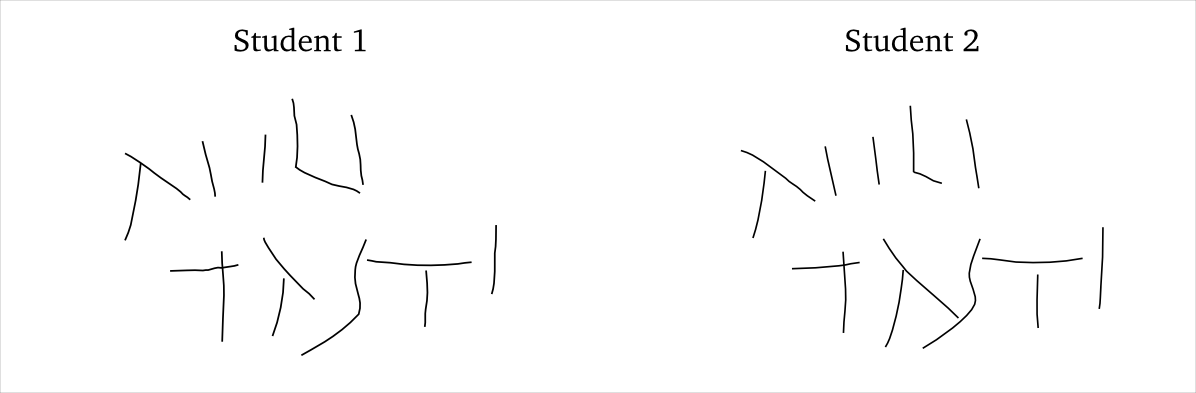
\includegraphics[scale=0.25]{EAGLE16lameetalteaching-img009.png}
\caption{12563 Obverse. The two students' reconstructions}
\label{fig:1}
\end{figure}

\begin{figure}[!bp]
\centering
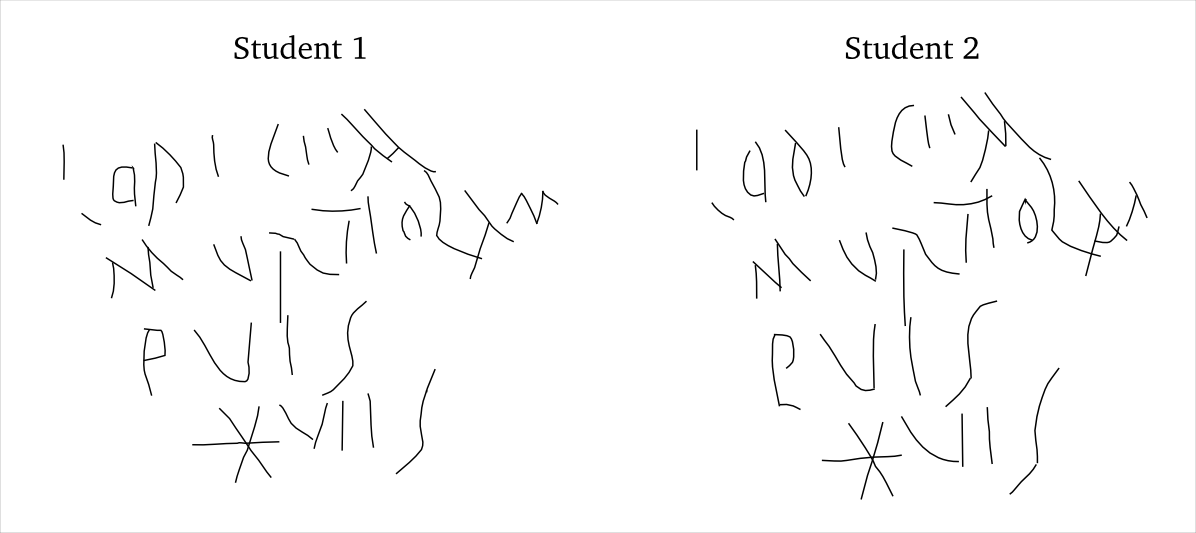
\includegraphics[scale=0.25]{EAGLE16lameetalteaching-img008.png}
\caption{12563 Reverse. The two students' reconstructions}
\label{fig:2}
\end{figure}



\subsection{Drawing \& Deciphering Without Help (obv. No. 13053)}


No. 13053 is an irregularly shaped rectangular lead tag with a damaged surface as well which makes the reading rather
uncertain. Besides the last, most recent inscription, one still discerns traces of older inscriptions. The reverse is
ignored. Students do not have neither transcriptions nor drawings.

%\begin{figure}
%\centering
%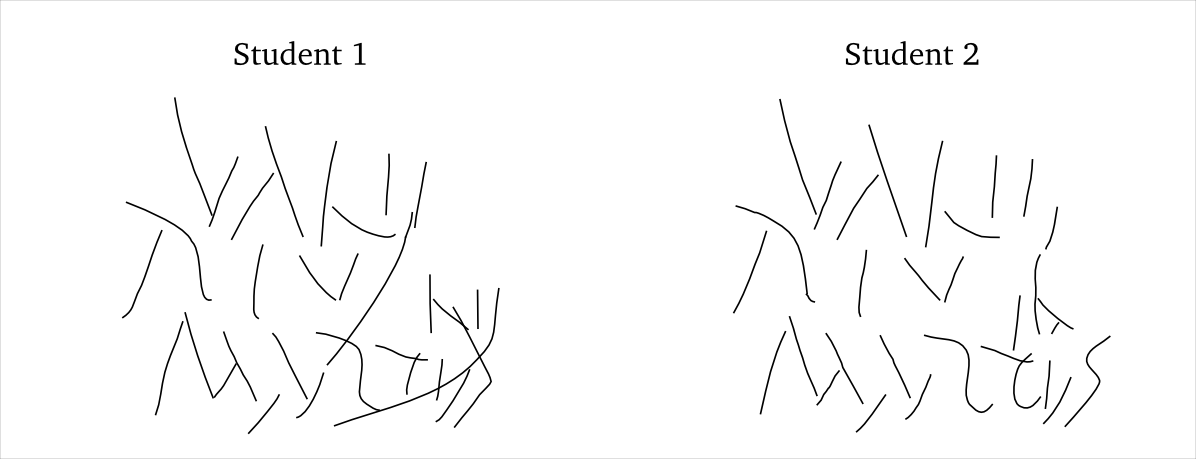
\includegraphics[width=2.009cm,height=1.96cm]{EAGLE16lameetalteaching-img010.png}
%\end{figure}
%\begin{figure}
%\centering
%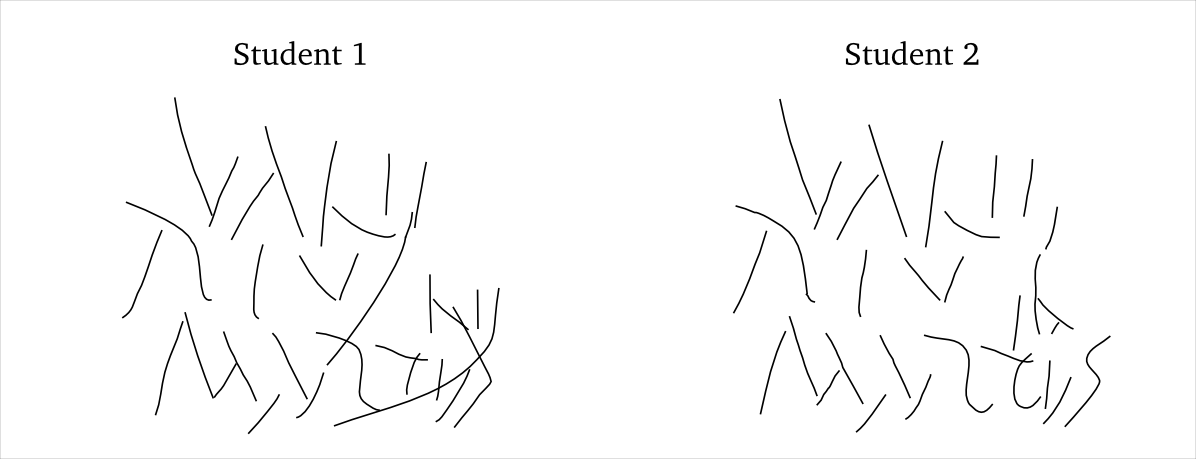
\includegraphics[width=2.103cm,height=1.961cm]{EAGLE16lameetalteaching-img010.png}
%\end{figure}
%\begin{figure}
%\centering
%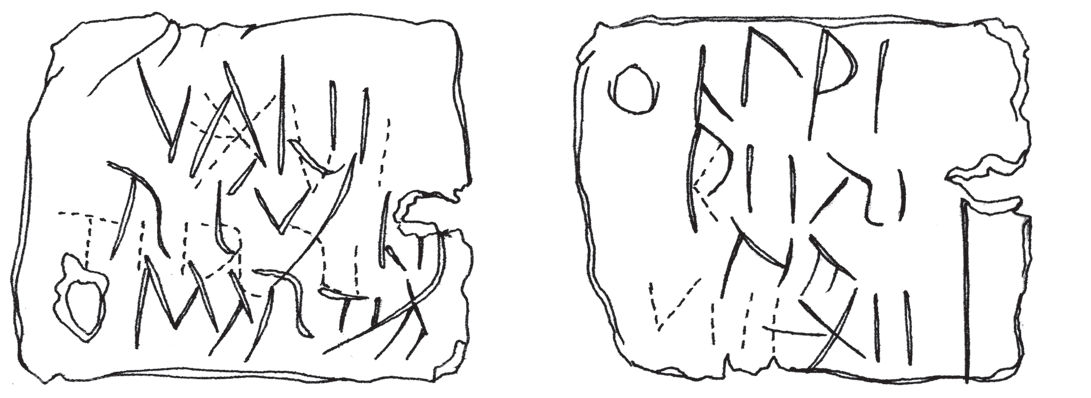
\includegraphics[width=2.044cm,height=1.794cm]{EAGLE16lameetalteaching-img011.png}
%\end{figure}

\begin{minipage}[t]{0.3\textwidth}
\textbf{Vale}\\
rius lis\\
Martia\\
\end{minipage}
\begin{minipage}[t]{0.3\textwidth}
(palimpsest)\\
\sout{X} \d{v}i\\
tiir \d{r} i\\
\end{minipage}
\begin{minipage}[c]{0.3\textwidth}
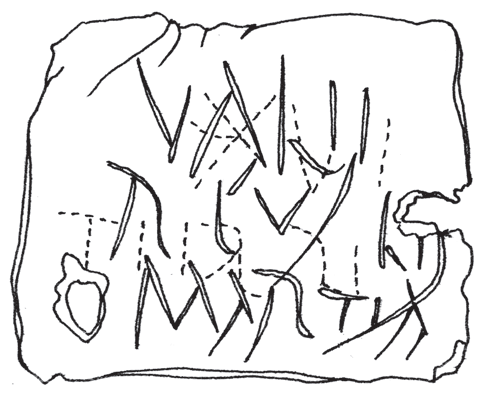
\includegraphics[scale=0.25]{EAGLE16lameetalteaching-img011a.png}
\end{minipage}



\begin{figure}[!bp]
\centering
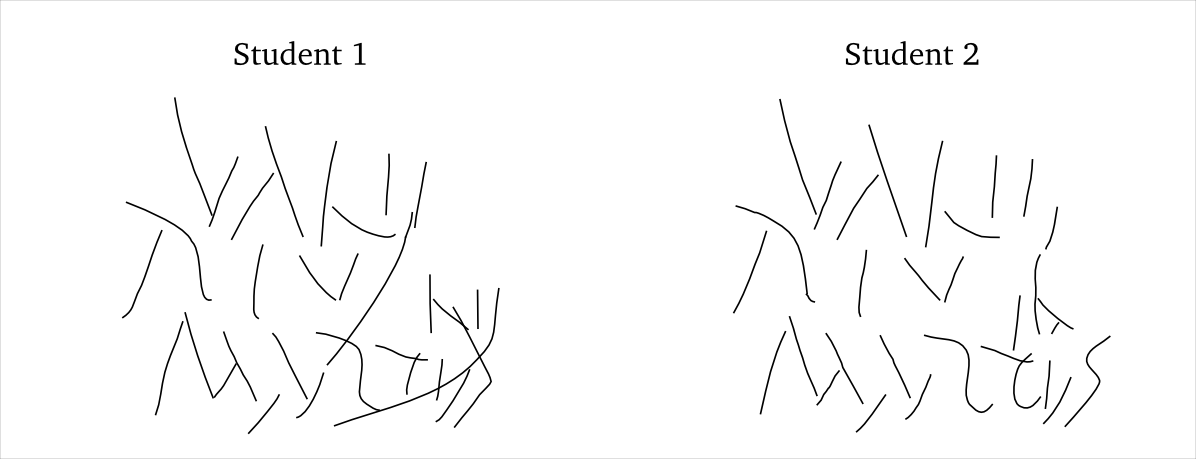
\includegraphics[scale=0.25]{EAGLE16lameetalteaching-img010.png}
\caption{13053 Obverse. Students' reconstructions}
\label{fig:3}
\end{figure}

The RTI file was presented to the students in an unusual reading position in order to reproduce the epigrapher’s initial
challenge of determining the proper orientation in which to read the lead tag. Students overcome this difficulty quite
quickly ({\textless}5 mn).

The last line, MARTIA, gave the student a hard time. Particularly the tail of the damaged S (end of the second line)
generates noise on the last letters.

\begin{table}
{\small
\addtolength{\tabcolsep}{-0.8mm}

\begin{tabular*}{\textwidth}{lllllllllllllll}
 & & & & & & & & & & & & & \\
\toprule
%\textbf{12563 (rev)} & \textbf{L} & \textbf{O} & \textbf{D} & \textbf{I} & \textbf{C} & \textbf{E} & \textbf{M} & & & & & &\\
%\midrule
%\textbf{Stud. 1} & \textit{L2} & \textit{O3} & \textit{D3} & \textit{I1} & \textit{C2} & \textit{E2} & \textit{M5} &  &  & & & & \\
%\textbf{Stud. 2} & \textit{?} & \textit{O3} & \textit{D5} & \textit{I2?} & \textit{C2} & \textit{E3} & \textit{M5} & & & & & &  \\
%\bottomrule
%\toprule
%& & & & & & & & & & & & & \\
%\midrule
\textbf{13053} & \textbf{V} & \textbf{A} & \textbf{L} & \textbf{E} & \textbf{R} & \textbf{I} & \textbf{U} & \textbf{S} & \textbf{M} & \textbf{A} & \textbf{R} & \textbf{T} & \textbf{I} & \textbf{A}\\ \midrule
\textbf{St. 1}& \textit{V2} & \textit{A10} & \textit{L3} & \textit{E3} & \textit{R7} & \textit{I2} & \textit{V1} & \textit{S6} & \textit{M5} & \textit{?} & \textit{R7} & \textit{T3} & \textit{?} & \textit{Ignored} \\
\textbf{St. 2}& \textit{V2} & \textit{A10} & \textit{L3} & \textit{E2} & \textit{R7} & \textit{I1} & \textit{V1} & \textit{S6?} & \textit{M5} & \textit{A10} & \textit{R6?} & \textit{T3?} & \textit{?I1} & \textit{A2} \\
\bottomrule
\end{tabular*}}

\caption{No. 13053 (obv).}
\label{tab:table2}
\end{table}


%begin{flushleft}
%tablefirsthead{}
%tablehead{}
%tabletail{}
%tablelasttail{}
%begin{supertabular}{|m{1.513cm}|m{0.37700003cm}|m{0.518cm}|m{0.361cm}|m{0.37700003cm}|m{0.37700003cm}|m{0.283cm}|m{0.37700003cm}|m{0.46900004cm}|m{0.439cm}|m{0.518cm}|m{0.518cm}|m{0.50200003cm}|m{0.297cm}|m{0.961cm}|}
%hline
%centering 13053 (obv.) &
%centering V &
%centering A &
%centering L &
%centering E &
%centering R &
%centering I &
%centering V &
%centering S &
%centering M &
%centering A &
%centering R &
%centering T &
%centering I &
%centering\arraybslash A\\\hline
%centering Stud. 1 &
%2 &
%10 &
%3 &
%3 &
%7 &
%2 &
%1 &
%6 &
%5 &
% &
%7 &
%3 &
% &
%gnored\\\hline
%centering Stud. 2 &
%2 &
%10 &
%3 &
%2 &
%7 &
%1 &
%1 &
%6? &
%5 &
%10 &
%6? &
%3? &
%1 &
%2\\\hline
%\end{supertabular}
%\end{flushleft}

\subsection{Palimpsest (obv. No. 13053)}



The older, erased layers, drawn with dashed lies on the drawings of the academic edition, are more difficult to read. No
g/t relationship between wSystem and tSystem was asked to students.

\begin{figure}[!bp]
\centering
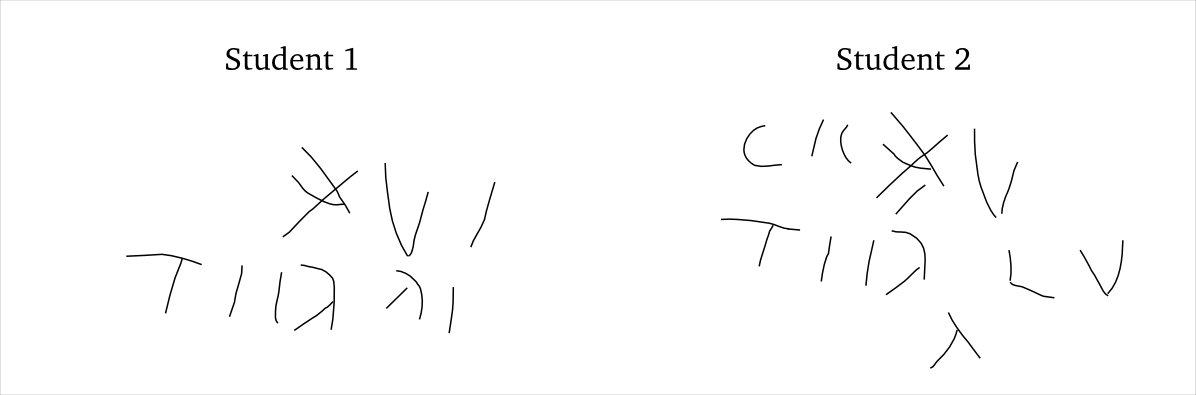
\includegraphics[scale=0.25]{EAGLE16lameetalteaching-img012.png}
\caption{12563 Obverse (palimpsest). The two students' reconstructions}
\label{fig:4}
\end{figure}


\section{Pedagogical Considerations}


\noindent From the educational standpoint, this pilot project succeeded tremendously. The students who undertook this
transcription in place of the usual research essay were, on average, far more motivated than their peers, and took
great pleasure and pride in their work. One student, whose cumulative grade at university to this point was below
average, excelled in this project and said that this was what he imagined university studies were going to be like. Two
others prepared a presentation based on this effort, and it was accepted as a 15 minute lecture at the university’s
annual undergraduate research seminar.

Some of the uncommon qualities of these materials made them particularly able to be studied by undergraduate students
with little or no Latin. The transcription of the tags’ oddly shaped letters was a skill that any person literate in a
Latin-script language (but not necessarily in Latin) could acquire. Indeed any additional understanding of Latin
grammar and syntax afford a reader little additional advantage, given the tags’ copious abbreviations. The tags’
frequent and regular use of symbols and numbers meant that the latin-less student could nevertheless quickly begin to
‘read’ the tags, or at least glean information from them.

However much the student researchers’ enthusiasm compensated, there were some impediments which will need to be removed
before a large number of students can undertake this work. To unilingual Anglophone students, the research materials on
the tags are daunting because little of it is available in English. Our volunteers were mostly bilingual Canadians who
could read French as well as English.

\section{Conclusion}


\noindent Gaining expertise with material remains requires time. When a museum trains students, this time is often limited due to
constrained facilities and personnel. In addition, the epigraphic material may be fragile and delicate: the less these
are manipulated by hands the best it is for their preservation. We believe that a process similar to the one described
here will allow us and others to train far more, wherever they may be in the world, while well preserving the
materials. It will represent a useful intermediary step that develops both epigraphic and digital skills. However,
adding such a step will require us to renew, in some regards, the way we train learners and to reconsider who teaches
what and how. The benefits of this renewal, though, would be many: it would ensure the transmission of epigraphic
tradition and the acquisition of good digital skills, whether to train eminent specialists or to allow access to the
roots of societies to the greatest number.

\section*{Aknowledgment}
\noindent We wish to acknowledge the research assistance of T. M. Crandall,
History student at Mount Allison University (Sackville, Canada), and C. Le Borgne, a Roman epigrapher and student of
M. Smith, who is Professor of Paleography at the École Nationale des Chartes and at the École Pratique des Hautes
Études (PSL Research University). His current seminar, for the Academic Year 2015/16, at the EPHE is entitled
``La lettre romaine, entre inscriptions monumentales et écritures communes''. The following
students at Mount Allison University participated in this experiment as part of their course work: D. Atkinson, E.
Beaton, M. Gillard, T. Hall and K. Wallace. We warmly thank M. Vazzana and C. Tanca, students of the Laurea
Specialistica in Informatica Umanistica at the University of Pisa, who prepared part of the great pedagogical material
as well as some useful didactic videos for the Laboratorio di Cultura Digitale. We are grateful to the Deutsches
Archäologisches Institut, and especially to Prof. R. Förtsch and to M. Romanello for offering us the opportunity to
present the DAP to the students of the Digital Classicist Berlin Seminar the 8th of December 2015.

\bibliographystyle{sapauth-eng}
\bibliography{../../EAGLE}

\end{document}
